% Created 2019-05-08 三 13:58
% Intended LaTeX compiler: pdflatex
\documentclass[11pt]{article}
\usepackage[utf8]{inputenc}
\usepackage[T1]{fontenc}
\usepackage{graphicx}
\usepackage{grffile}
\usepackage{longtable}
\usepackage{wrapfig}
\usepackage{rotating}
\usepackage[normalem]{ulem}
\usepackage{amsmath}
\usepackage{textcomp}
\usepackage{amssymb}
\usepackage{capt-of}
\usepackage{hyperref}
\usepackage{minted}
\usepackage{commath,amsmath}
\newcommand{\bl}[1] {\boldsymbol{#1}}
\graphicspath{{../../images/ArtificialIntelligence/}}
\author{wu}
\date{\today}
\title{Artificial Intelligence}
\hypersetup{
 pdfauthor={wu},
 pdftitle={Artificial Intelligence},
 pdfkeywords={},
 pdfsubject={},
 pdfcreator={Emacs 26.1 (Org mode 9.1.14)}, 
 pdflang={English}}
\begin{document}

\maketitle
\tableofcontents

\section{Inference and Reasoning}
\label{sec:orgecdf97d}
\subsection{Propositional logic}
\label{sec:org04dde97}
\subsection{Predicate logic}
\label{sec:org811b44f}
\subsection{First Order Inductive Learner}
\label{sec:org4d41dbe}
\textbf{knowledge graph}: node = entity, edge = relation.
triplet (head entity, relation, tail entity)
\section{Statistical learning and modeling}
\label{sec:org6127c05}
\subsection{Machine Learning: the concept}
\label{sec:org48fc292}
\subsubsection{Example and concept}
\label{sec:org68e6bfa}
\begin{description}
\item[{Supervised learning problems}] applications in which the \textbf{training data} comprises examples of the input
vectors along with their corresponding \textbf{target vectors} are known

classification and regression
\item[{Unsupervised learning problems}] the training data consists of a set of input vectors X \textbf{without any
corresponding target values}

density estimation, clustering, hidden markov models
\item[{Reinforcement learning problem}] finding suitable actions to take in a given situation in order to
maximize a reward. Here the learning algorithm is not given examples of
optimal outputs, in contrast to supervised learning, but must instead
discover them by a process of trial and error. A general feature of
reinforcement learning is the trade-off between exploration and exploitation
\end{description}

types of machine learning
\begin{itemize}
\item supervised learning
\begin{itemize}
\item classification: the output is categorical or nominal variable
\item regression: the output is read-valued variable
\end{itemize}
\item unsupervised learning
\item semi-supervised learning
\item reinforcement learning
\item deep learning
\end{itemize}
\subsubsection{supervised learning: important concepts}
\label{sec:org88d88e7}
\begin{itemize}
\item Data: labeled instances \(<\bl{x}_i,\bl{y}>\)
\item features: attribute-value pairs which characterize each \(\bl{x}\)
\item learning a discrete function: \textbf{classification}
\item learning a continuous function: \textbf{regression}
\end{itemize}

\textbf{Classification} - A two-step process
\begin{itemize}
\item \textbf{model construction}
\item \textbf{model usage}
\end{itemize}

\textbf{regression}
\begin{itemize}
\item Example: price of a used car

\(\bl{x}\): car attributes. \(\bl{y}=g(\bl{x}\mid\bl{\theta})\): price. \(g\):
model. \(\theta\) parameter set.
\end{itemize}
\subsection{example: polynomial curve fitting}
\label{sec:org97bf6ea}
\subsection{probability theory review and notation}
\label{sec:org861f6ea}
rules of probability
\begin{itemize}
\item \textbf{sum rule} \(p(X)=\displaystyle\sum_Yp(X,Y)\)
\item \textbf{product rule} \(p(X,Y)=p(Y|X)p(X)\)
\end{itemize}

Bayes' Theorem: \(p(Y|X)=\frac{p(X|Y)p(Y)}{p(X)}\). Using sum rule
\(p(X)=\displaystyle\sum_Yp(X|Y)p(Y)\)

probability densities. 
\begin{align*}
p(x\in(a,b))&=\int_a^bp(x)dx\\
P(z)&=\int_{-\infty}^z p(x)dx\\
\int_{-\infty}^\infty p(x)dx&=1\quad p(x)\le0
\end{align*}


\textbf{expectation} \(\mathbb{E}[f]=
   \begin{cases}
   \displaystyle\sum_{x}p(x)f(x) & \text{discrete variables}\\
   \int p(x)f(x)dx & \text{continuous variables}
   \end{cases}\). In either cases,
\(\mathbb{E}[f]\approx\frac{1}{N}\displaystyle\sum_{n=1}^N f(x_n)\).
\textbf{conditional expectation}: \(\mathbb{E}_x[f| y]=\displaystyle\sum_xp(x| y)f(x)\).

The \textbf{variance} of \(f(x)\) is

\begin{align*}
var[f]&=\mathbb{E}[(f(x)-\mathbb{E}[f(x)])^2]\\
&=\mathbb{E}[f(x)^2-2f(x)\mathbb{E}[f(x)]+\mathbb{E}[f(x)]^2]\\
&=\mathbb{E}[f(x)^2]-\mathbb{E}[f(x)]^2
\end{align*}


   The \textbf{covarian
ce} is

\begin{align*}
cov[x,y]&=\mathbb{E}_{x,y}[(x-\mathbb{E}[x])(y-\mathbb{E}[y])]\\
&=\mathbb{E}_{x,y}[xy]-\mathbb{E}[x]\mathbb{E}[y]
\end{align*}


\emph{the variance of the sum of two independent random variables is the sum of}
\emph{variance}. Given
\begin{center}
\begin{tabular}{c|c}
X & probability\\
\hline
\(x_1\) & \(p_1\)\\
\(\dots\) & \(\dots\)\\
\(x_n\) & \(p_n\)\\
\end{tabular}
\end{center}

\begin{center}
\begin{tabular}{c|c}
Y & probability\\
\hline
\(y_1\) & \(q_1\)\\
\(\dots\) & \(\dots\)\\
\(y_m\) & \(q_m\)\\
\end{tabular}
\end{center}
\begin{align*}
var(X+Y)=var(X)+var(Y)
\end{align*}

In case of two vectors of random variables \(\bl{x}\) and \(\bl{y}\), the
covariance is a matrix
\begin{align*}
cov[\bl{x},\bl{y}]&=\mathbb{E}_{\bl{x},\bl{y}}[(\bl{x}-\mathbb{E}[\bl{x}])(\bl{y}^T
-\mathbb{E}[\bl{y}^T])]\\
&=\mathbb{E}_{\bl{x},\bl{y}}[\bl{xy}^T]-\mathbb{E}[\bl{x}]\mathbb{E}[\bl{y}^T]
\end{align*}

\textbf{Bayesian probabilities}: \(P(A|B)=\frac{P(B|A)P(A)}{P(B)}\). For a data set 
\(\mathcal{D}=\{t_1,\dots,t_n\}\) and assumption \(w\),
\(p(w|\mathcal{D})=\frac{p(\mathcal{D}|w)p(w)}{p(\mathcal{D})}\). \(p(w)\) is
\textbf{prior probability}, \(p(\mathcal{D}|w)\) is \textbf{likelihood} (the probability
\(\mathcal{D}\) happens). Hence 
\begin{equation*}
\text{posterior}\propto\text{likelihood}\times\text{prior}
\end{equation*}

\textbf{Gaussian distribution}.
\begin{equation*}
\mathcal{N}(x|\mu,\sigma^2)=\frac{1}{(2\pi\sigma^2)^{1/2}}\exp\left\{
-\frac{1}{2\sigma^2}(x-\mu)^2\right\}
\end{equation*}
\(\mu\) is called \textbf{mean}, \(\sigma^2\) is called \textbf{variance}, \(\sigma\) \textbf{standard
deviation}, \(\beta=1/\sigma^2\) \textbf{precision}
\begin{align*}
\mathbb{E}[x]&=\int_{-\infty}^\infty\mathcal{N}(x|\mu,\sigma^2)xdx=\mu\\
\mathbb{E}[x^2]&=\int_{-\infty}^\infty\mathcal{N}(x|\mu,\sigma^2)x^2dx=\mu^2
+\sigma^2\\
var[x]&=\mathbb{E}[x^2]-\mathbb{E}[x]^2=\sigma^2\\
\end{align*}
For \$D\$-dimensional vector \(\bl{x}\) of continuous variables
\begin{equation*}
\mathcal{N}(\bl{x}|\bl{\mu},\bl{\Sigma})=\frac{1}{(2\pi)^{D/2}}\frac{1}
{\abs{\bl{\Sigma}}^{1/2}}\exp\left\{-\frac{1}{2}(\bl{x}-\bl{\mu})^T
\bl{\Sigma^{-1}}(\bl{x}-\bl{\mu})\right\}
\end{equation*}

To determine values for the unknown parameters given \(\mu\) and \(\sigma^2\) by
maximizing the likelihood function. Use log.
\begin{align*}
P(\bl{X}|\mu,\sigma^2)&=\displaystyle\prod_{n=1}^N\mathcal{N}(x_n|\mu,\sigma^2)\\
\Rightarrow \ln P(\bl{X}|\mu,\sigma^2)&=-\frac{1}{2\sigma^2}
\displaystyle\sum_{n=1}^N(x_n-\mu)^2-\frac{N}{2}\ln\sigma^2-\frac{N}{2}\ln(2\pi)\\
\end{align*}
Hence \(\mu_{ML}=\frac{1}{N}\displaystyle\sum_{n=1}^Nx_n\),
\(\sigma^2_{ML}=\frac{1}{N}\displaystyle\sum_{n=1}^N(x_n-\mu_{ML})^2\) by
partial derivative. Maximum likelihood estimator for mean is unbiased, that
is, \(\mathbb{E}(\mu_{ML})=\mu\). Maximum likelihood estimator for variance is
biased. \(\mathbb{E}(\sigma_{ML}^2)=\mathbb{E}(x^2)-\mathbb{E}(\mu_{ML}^2)=
   \frac{N-1}{N}\sigma_x^2\)
\subsection{information theory}
\label{sec:org7cdc09b}
\textbf{entropy}: measuring uncertainty of a random variable \(X\).
\(H(X)=H(p)=-\displaystyle\sum_{x\in\Omega}p(x)\log p(x)\) where \(\Omega\) is
all possible values and define \(0\log0=0,\log=\log_2\)

\(H(X)=\displaystyle\sum_{x\in\Omega}p(x)\log_2\frac{1}{p(x)}=
   E(\log_2\frac{1}{p(x)})\). And "information of \(x\)"​="\#bits to code \(x\)"​=\(-\log
   p(x)\)

\textbf{Kullback-Leibler divergence}: comparing two distributions
\subsection{model selection}
\label{sec:org959b873}
\textbf{cross-validation}
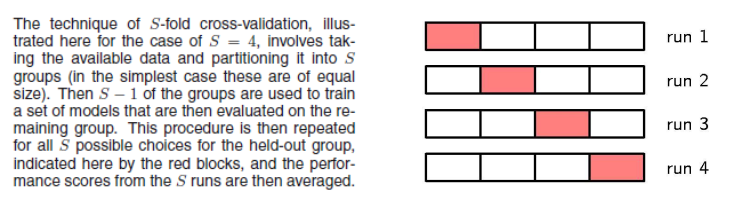
\includegraphics[width=100mm]{CrossValidation}

split training data into \textbf{training set} and \textbf{validation set}. Train different
models on training set and choose model with minimum error on validation set.
\subsection{decision theory}
\label{sec:orgbf5ea6e}
Suppose we have an input vector \(\bl{x}\) together with a corresponding vector
\(\bl{t}\) of target variables and our goal is to predict \(\bl{t}\) given new
value for \(\bl{x}\). The joint probability distribution \(p(\bl{x},\bl{t})\)
provides a complete summary of the uncertainty with these variables
\section{Statistical learning and modeling - Supervised learning}
\label{sec:orgf3463ed}
\subsection{Basic concepts}
\label{sec:orgf751c3e}
\begin{itemize}
\item \textbf{Linearly separable}
\begin{itemize}
\item decision regions:

input space is divided into several regions
\item decision boundaries:
\begin{itemize}
\item under linear models, it's a linear function
\item (D-1)-dimensional hyper-plane within the D-dimensional input space
\end{itemize}
\end{itemize}
\item \textbf{representation of class labels}
\begin{itemize}
\item Two classes K = 2
\item K classes
\begin{itemize}
\item 1-of-K coding scheme \(\bl{t}=(0,0,1,0,0)^T\)
\end{itemize}
\item Predict discrete class labels
\begin{itemize}
\item linear model prediction \(y(\bl{x})=\bl{w}^T\bl{x}+w_0\)
w: weight vector, w\(_{\text{0}}\) bias/threshold
\item nonlinear function \(f(.):R\to(0,1)\)
\item generalized linear models
\(y(\bl{x})=f(\bl{w}^T\bl{x}+w_0)\)
f:activation function
\item dicision surface
\(y(\bl{x})=\text{constant}\to \bl{w}^T\bl{x}+w_0=\text{constant}\)
\end{itemize}
\end{itemize}
\item \textbf{Three classification approaches}
\begin{itemize}
\item discriminant function
\begin{itemize}
\item least squares approach
\item fisher's linear discriminant
\item the perceptron algorithm of rosenblatt
\end{itemize}
\item use discriminant functions directly and don't compute probabilities

Given discriminant functions \(f_1(\bl{x}),\dots,f_K(\bl{x})\). Classify
\(\bl{x}\) as class \(\mathcal{C}_k\) iff \(f_k(\bl{x})>f_j(\bl{x}),\forall
       j\neq k\)

\begin{itemize}
\item \textbf{least-squares approach}: making the model predictions as close as
possible to a set of target values
\item \textbf{fisher's linear discriminant}: maximum class separation in the ouput
space
\item \textbf{the perceptron algorithm of rosenblatt}
\end{itemize}
\item generative approach
\begin{itemize}
\item model the class-conditional densities and the class priors
\item compute posterior probabilities through Bayes's theorem

\(\underbrace{p(\mathcal{C}_k|\bl{x})}_\text{posterior for class}=
         \frac{\overbrace{p(\bl{x}|\mathcal{C}_k)}^\text{class conditional density}
         \overbrace{p(\mathcal{C}_k)}^\text{class prior}}{p(\bl{x})}=
         \frac{p(\bl{x}|\mathcal{C}_k)p(\mathcal{C}_k)}{\sum_{j}p(\bl{x}|\mathcal{C}_j)
         p(\mathcal{C}_j)}\)
\end{itemize}
\end{itemize}
\end{itemize}
\subsection{discriminant functions}
\label{sec:org4fa00aa}
\subsubsection{Two classes}
\label{sec:org0e90dbf}
\begin{itemize}
\item Linear discriminant function \(y(\bl{x})=\bl{w}^T\bl{x}+w_0\)
\begin{itemize}
\item Dicision surface \(\Omega:y(\bl{x})=0\)
\item the normal distant from the origin to the dicision surface
\(\frac{\bl{w}^T\bl{x}}{\norm{\bl{w}}}=-\frac{w_0}{\norm{\bl{w}}}\)
\item if \(x_A,x_B\) lie on the decision surface \(y(\bl{x}_A)=y(\bl{x}_B)=0\),
then \(\bl{w}^T(\bl{x}_A-\bl{x}_B)=0\). hence w is orthogonal to every
vector lying within Ω. \(\frac{\bl{w}}{\norm{\bl{w}}}\) is the normal
vector of Ω

\item \(\bl{x}=\bl{x}_\perp+r\frac{\bl{w}}{\norm{\bl{w}}}\) hence
\(r=\frac{y(\bl{x})}{\norm{\bl{w}}}\). \(y(\bl{x}_\perp)=0\to
        \bl{w}^T\bl{x}=-w_0+r\frac{\bl{w}^T\bl{w}}{\norm{\bl{w}}}\)
\item \(\tilde{\bl{w}}=(w_0,\bl{w}), \tilde{\bl{x}}=(x_0,\bl{x}),
        y(\bl{x})=\tilde{\bl{w}}^T\tilde{\bl{x}}\)
\end{itemize}
\end{itemize}
\subsubsection{K-class}
\label{sec:orgfd6ece7}
\begin{itemize}
\item One-versus-the-rest classifier
K - 1 classifiers each of which solves a two-class problem
\item One-versus-one classifier
K(K-1)/2 binary discriminant functions
\item single K-class discriminant comprising K linear functions
\(y_k(\bl{x})=\bl{w}_k^T\bl{x}+w_{k_0}\)
\begin{itemize}
\item assigning a point x to class \(\mathcal{C}_k\) if
\(y_k(\bl{x}>y_j(\bl{x}))\) for all j≠k
\item dicision boundary between class \(\mathcal{C}_k, \mathcal{C}_j\) is given
\(y_k(\bl{x})=y_j(\bl{x})\to
        (\bl{w}_k-\bl{w}_j)^T\bl{x}+(w_{k_0}-w_{j_0})=0\)
\item \(\mathcal{R}_k\) is singly connected convex
\item \(\hat{\bl{x}}=\lambda\bl{x}_A+(1-\lambda)\bl{x}_B\) where \(0\le\lambda\le
        1\), \(y_k(\hat{\bl{x}})=\lambda y_k(\bl{x}_A)+(1-\lambda)y_k(\bl{x}_B)\)
and hence \(\hat{x}\) also lies inside \(\mathcal{R}_k\)
\end{itemize}
\end{itemize}
\subsubsection{Learning the parameters of linear discriminant functions}
\label{sec:org703237f}
\begin{enumerate}
\item Linear basis function models
\label{sec:orgb69b6dc}
\textbf{linear regression}:
\(y(\bl{x},\bl{w})=w_0+w_1x_1+\dots+w_Dx_D=\bl{w}^T\bl{x}\).

For nonlinear functions \(\phi_j\),
\(y(\bl{x},\bl{w})=w_0+\displaystyle\sum_{j=1}^{M-1}
     w_j\phi_j(\bl{x})=\bl{w}^T\bl{\phi(\bl{x})}\) where \(\phi_j(\bl{x})\) are
\textbf{basis functions} 
\item \textbf{parameter optimization via maximum likelihood}
\label{sec:org403f5af}

Assume target variable \(t\) is given by a deterministic function
\(y(\bl{x},\bl{w})\) with additive Gaussian noice so that
\(t=y(\bl{x},\bl{w})+\epsilon\) where \(\epsilon\) is a zero mean Gaussian
random variable with precision \(\beta\), hence we can write
\begin{equation*}
p(t|\bl{x},\bl{w},\beta)=\mathcal{N}(t|y(\bl{x},\bl{w}),\beta^{-1})
\end{equation*}
and \(\mathbb{E}(t|\bl{x})=\int tp(t|\bl{x})dt=y(\bl{x},\bl{w})\)

For data set \(\bl{X}=\{\bl{x}_1,\dots,\bl{x}_n\},\bl{t}=(t_1,\dots,t_n)^T\),
\(p(t|\bl{X},\bl{w},\beta)=\displaystyle\prod_{n=1}^N\mathcal{N}(t_n|
     \bl{w}^T\bl{\phi}(\bl{x}_n),\beta^{-1})\)

\(\ln p(t|\bl{w},\beta)=\displaystyle\sum_{n=1}^N\ln\mathcal{N}(t_n|
     \bl{w}^T\bl{\phi}(\bl{x}_n),\beta^{-1})=\frac{N}{2}\ln\beta-\frac{N}{2}\ln(2\pi)-
     \beta E_D(\bl{w})\)

\(E_D(\bl{w})=\frac{1}{2}\displaystyle\sum_{n=1}^N
     \left\{t_n-\bl{w}^T\bl{\phi}(\bl{x}_n)\right\}^2=
     \frac{1}{2}\norm{t-\Phi\bl{w}}\) is sum-of-squares error function

solve \(\bl{w}\) by maximum likelihood.
\begin{equation*}
\nabla\ln p(\bl{t}|\bl{w},\beta)=\displaystyle\sum_{n=1}^N
\left\{t_n-\bl{w}^T\bl{\phi}(\bl{x}_n)\right\}\phi(\bl{x}_n)^T
\end{equation*}
\begin{equation*}
0=\displaystyle\sum_{n=1}^N t_n\bl{\phi}(\bl{x}_n)^T-\bl{w}^T
(\displaystyle\sum_{n=1}^N\bl{\phi}(\bl{x}_n)\bl{\phi}(\bl{x}_n)^T)
\end{equation*}
Hence we get
\begin{equation*}
\bl{w}_{ML}=(\bl{\Phi}^T\bl{\Phi})^{-1}\bl{\Phi}^T\bl{t}
\end{equation*}
\(\Phi\) is \textbf{design matrix}.
\[
\Phi=\begin{pmatrix}
 \phi_0(\bl{x}_1) & \phi_1(\bl{x}_1) & \dots & \phi_{M-1}(\bl{x}_1) \\
 \phi_0(\bl{x}_2) & \phi_1(\bl{x}_2) & \dots & \phi_{M-1}(\bl{x}_2) \\
 \vdots & \vdots & \ddots & \vdots \\
 \phi_0(\bl{x}_N) & \phi_1(\bl{x}_N) & \dots & \phi_{M-1}(\bl{x}_N) \\
\end{pmatrix}
\]

For bias parameter \(w_0\).
\(E_D(\bl{w})=\frac{1}{2}\displaystyle\sum_{n=1}^N 
     \{t_n-w_0-\displaystyle\sum_{j=1}^{M-1}w_j\phi_j(\bl{x}_n)\}^2\). Hence
\(w_0=\bar{t}-\displaystyle\sum_{j=1}^{M-1}w_j\bar{\phi_j}\),
\(\bar{t}=\frac{1}{N}\displaystyle\sum_{n=1}^Nt_n\),
\(\bar{\phi_j}=\frac{1}{N}\displaystyle\sum_{n=1}^N\phi_j(\bl{x}_n)\).

\(frac{N}{2\beta}=E_D(\bl{w})\). \(\frac{1}{\beta_{ML}}=
     \frac{1}{N}\displaystyle\sum_{n=1}^N\left\{t_n-\bl{w}^T_{ML}
     \bl{\phi}(\bl{x}_n)\right\}^2\)
\item Least-squares approach
\label{sec:org3a414e4}
\begin{itemize}
\item Problem
\begin{itemize}
\item Each class \(\mathcal{C}_k\) is described by its own linear model 
\(y_k(\bl{x})=\bl{w}_k^T\bl{x}+w_{k0}\)
\item group together: \(y(\bl{x})=\widetilde{\bl{W}}^T\tilde{\bl{x}}\),
\(\tilde{\bl{w}}_k=(w_{k0},\bl{w}_k^T)^T\), \(\tilde{\bl{x}}=(1,\bl{x}^T)^T\)
\end{itemize}
\item Learning
\begin{itemize}
\item minimizing SSE function sum-of-squares
\(SSE=\displaystyle\sum_{i=1}^n(y_i-f(x_i))^2\)
\(E_D(\widetilde{\bl{W}})=1/2\text{Tr}\{(\bl{\widetilde{X}\widetilde{W}-T})^T 
         (\bl{\widetilde{X}\widetilde{W}-T})\}\)

\(\bl{\widetilde{W}}=(\bl{\widetilde{X}}^T\bl{\widetilde{X}})^{-1}\bl{\widetilde{X}}^T\bl{T}\)
\end{itemize}
\end{itemize}
\item fisher's linear discriminant
\label{sec:org77ad6be}

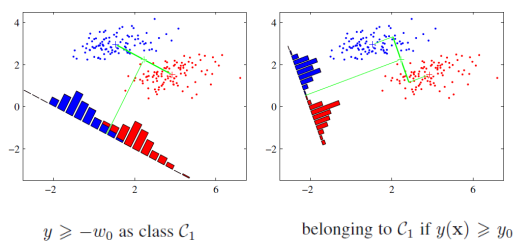
\includegraphics[width=100mm]{Fisher}

from the view of dimensionality reduction
\(y\ge -w_0\) as class \(\mathcal{C}_1\)

\(m_1=\frac{1}{N_1}\displaystyle\sum_{n\in\mathcal{C}_1}x_n, 
     m_2=\frac{1}{N_2}\displaystyle\sum_{n\in\mathcal{C}_2}x_n
     \xrightarrow{y=\bl{w}^T\bl{x}} m_2-m_1=\bl{w}^T(\bl{m}_2-\bl{m}_1)\)
\item the perceptron algorithm of rosenblatt
\label{sec:org636bbc8}
\end{enumerate}
\subsection{probalibilistic generative models}
\label{sec:orgda0dcd5}
A probabilistic view of classification from simple assumptions about the
distribution of the data

\begin{align*}
p(\mathcal{C}_1|\bl{x})&=\frac{p(\bl{x}|\mathcal{C}_1)p(\mathcal{C}_1)}
{p(\bl{x}|\mathcal{C}_1)p(\mathcal{C}_1)+p(\bl{x}|\mathcal{C}_2)p(\mathcal{C}_2)}\\
&=\frac{1}{1+\exp(-a)}=\sigma(a)
\end{align*}
where 
\begin{equation*}
a=\ln\frac{p(\bl{x}|\mathcal{C}_1)p(\mathcal{C}_1)}
{p(\bl{x}|\mathcal{C}_2)p(\mathcal{C}_2)}
\end{equation*}
and \(\sigma(a)\) is the \textbf{logistic sigmoid} function defined by
\begin{equation*}
\sigma(a)=\frac{1}{1+\exp(-a)}
\end{equation*}
and \(\sigma(-a)=1-\sigma(a)\), its inverse is \textbf{logit} function
\begin{equation*}
a=\ln(\frac{\sigma}{1-\sigma})
\end{equation*}

For case of \(K > 2\) classes, we have the following \textbf{multi-class generalization}
\begin{equation*}
p(\mathcal{C}_k|\bl{x})=\frac{p(\bl{x}|\mathcal{C}_k)p(\mathcal{C}_k)}
{\sum_jp(\bl{x}|\mathcal{C}_j)p(\mathcal{C}_j)}=\frac{\exp(a_k)}{\sum_j\exp(a_j)},
a_k=\ln\left[p(\bl{x}|\mathcal{C}_k)p(\mathcal{C}_k)\right]
\end{equation*}
The \textbf{normalized exponential} is known as the \textbf{softmax function} as it represents
a \emph{smoothed version of the max function}
\begin{equation*}
\text{if } a_k\ll a_j,\forall j\neq k,\text{then } p(\mathcal{C}_k|\bl{x})\approx 1,
p(\mathcal{C}_j|\bl{x})\approx 0
\end{equation*}

For \textbf{continuous inputs}, assume
\begin{equation*}
p(\bl{x}|\mathcal{C}_k)=\frac{1}{(2\pi)^{D/2}}\frac{1}
{\abs{\bl{\Sigma}}^{1/2}}\exp\left\{-\frac{1}{2}(\bl{x}-\bl{\mu}_k)^T
\bl{\Sigma^{-1}}(\bl{x}-\bl{\mu}_k)\right\}
\end{equation*}
\begin{enumerate}
\item 2 classes
\begin{align*}
p(\mathcal{C}_1|\bl{x})&=\sigma(\bl{w}^T\bl{x}+w_0)\\
\bl{w}&=\bl{\Sigma}^{-1}(\bl{\mu}_1-\bl{\mu}_2)\\
w_0&=-\frac{1}{2}\bl{\mu}_1^T\bl{\Sigma}^{-1}\bl{\mu}_1+
\frac{1}{2}\bl{\mu}_2^T\bl{\Sigma}^{-1}\bl{\mu}_2+\ln\frac{p(\mathcal{C}_1)}
{p(\mathcal{C}_2)}\\
\end{align*}
\item K classes
\begin{align*}
a_k(\bl{x})&=\bl{w}_k^T\bl{x}+w_{k0}\\
\bl{w}_k&=\bl{\Sigma}^{-1}\bl{\mu}_k\\
w_{k0}&=-\frac{1}{2}\bl{\mu}_k^T\bl{\Sigma}^{-1}\bl{\mu}_k+\ln p(\mathcal{C}_k)
\end{align*}
\end{enumerate}
\subsection{probabilistic discriminative models}
\label{sec:org24cf01a}
\subsection{Boosting}
\label{sec:org81a853a}
Originally designed for classification problems.

Motivation: a procedure that combines the outputs of many "weak" classifiers
to produce a strong/accurate classifier


\subsubsection{AdaBoost}
\label{sec:orgd9fad99}
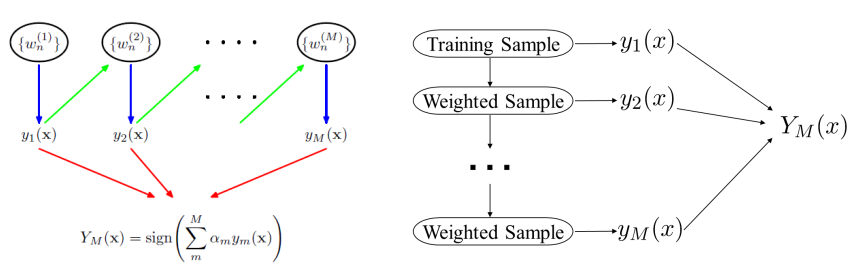
\includegraphics[width=100mm]{Boosting}
\section{wef}
\label{sec:org9d6192f}
\subsection{wfe}
\label{sec:org3180259}
K-means
\end{document}